\documentclass[11pt]{beamer}
\usetheme{default}
\usecolortheme{rose}
\setbeamertemplate{headline}
{%
	\hfill\makebox(0,-2)[rt]{\insertlogo}%
}
\setbeamertemplate{sidebar right}
{%
	\vfill%
	\llap{\usebeamertemplate***{navigation symbols}\hskip0.1cm}%
	\vskip2pt%
}
\setbeamertemplate{caption}[numbered]

\usepackage[utf8]{inputenc}
\usepackage[T1]{fontenc}
\usepackage[portuguese]{babel}
\usepackage{amsmath}
\usepackage{amsfonts}
\usepackage{amssymb}
\usepackage{graphicx}

\author{Group No. 8 \\ Group members: Li Mingyang,  Guo Junjie, Wu Heyue, Yang Buhan}
\title{Statistics of Financial Markets \\
	Project 4}
\date{July 20, 2016}
%\subtitle{}
\logo{\includegraphics[width=2.4cm,height=1.6cm]{WISE}}
%\institute{}
%\date{}
%\subject{}
%\setbeamercovered{transparent}
%\setbeamertemplate{navigation symbols}{}

\begin{document}
	\maketitle
	
	\section*{Outline}
		\begin{frame}
	    	\tableofcontents
    	\end{frame}
    	
    \section{An Introduction to CIR Model}
    \section{Bond Pricing with CIR model}
    \section{Calibrating the CIR Model}
    \section{Spot Rate Series and Term Structure}
	
	%first page
	\begin{frame}
		\frametitle{CIR Model}
		\begin{definition}
			In \alert{Cox, Ingersoll, Roll (CIR) Model}, the short-rate satisfies the SDE
			\begin{align}
			dr(t)=a\{b-r(t)\}dt+\sigma \sqrt{r(t)}dW_t
			\end{align}
			where a, b, $ \sigma $ are constants and $ W_t $ is a Wiener process.
		\end{definition}
		
		\begin{itemize}
			\item proposed by Cox, Ingersoll and Ross (1985)
			\item equilibrium spot rate model
            \item mean reversion
			\item nonnegative r(t) if $ 2ab\geq\sigma^2 $
		\end{itemize}
		
	\end{frame}
	
	%second page
	\begin{frame}
		\frametitle{Bond Pricing with CIR model}
		Under the corresponding numeraire:
		\[
		V(t,T)=E_t[exp\{-\int_{t}^{T}r(s)ds\}V(T,T)]
		\]
		with
		\[
		dr(t)=\mu_rdt+\sigma_rdW_t
		\]
		and
		\[
		\mu_r=\mu\{r(t),t\}, \, \sigma_r=\sigma\{r(t),t\}
		\]
	\end{frame}
	
	%third page
	\begin{frame}
		\frametitle{Bond Pricing with CIR model}
		By means of the condition that $ V(T,T)=1 $, in combination with $ It\hat{o}'s  \,Lemma $ we get:
		\begin{multline}
		dV(T,T)=\{\frac{\partial V(t,T)}{\partial t}+\frac{1}{2}\sigma^2\frac{\partial^2V(t,T)}{\partial r^2}+ \\
                \mu_r\frac{\partial V(t,T)}{\partial r}\}dt+\sigma\frac{\partial V(t,T)}{\partial r}dW_t
		\end{multline}
		under the risk-neutral measure the PDE of the CIR model is:
		\begin{equation}
		r(t)V(t,T)= \frac{\partial V(t,T)}{\partial t} + \frac{1}{2}r(t)\sigma^2\frac{\partial^2 V(t,T)}{\partial r^2}+ a\{b-r(t)\}\frac{\partial V(t,T)}{\partial r}
        \end{equation}
	\end{frame}
	
	%4th page
	\begin{frame}
		\frametitle{Bond Pricing with CIR model}
		Assuming $ V(t,T)=exp\{A(t)-r(t)B(t)\} $ and a nominal value 1, we can consider:
		\begin{align*}
		\frac{\partial V(t,T)}{\partial t}=& \{A'(t)-r(t)B'(t)\}V(t) \\
		\frac{\partial V(t,T)}{\partial r}=& -B(t)V(t) \\
		\frac{\partial^2 V(t,T)}{\partial r^2}=& B^2(t)V(t)
		\end{align*}
	\end{frame}
	
	%5th page
	\begin{frame}
		\frametitle{Bond Pricing with CIR model}
		With the boundary conditions $ V(T,T)=1 $ and $ A(T,T)=B(T,T)=0 $:
		\[
		V(t,T)=exp\{A(t)-r(t)B(t)\}
		\]
		where
		\begin{align*}
		A(t)=& \frac{2ab}{\sigma^2}log\frac{2\psi \,exp\{(a+\psi)(T-t)/2\}}{2\psi+(a+\psi)exp\{\psi(T-t)-1\}} \\
		B(t)=& \frac{2exp\{\psi(T-t)-1\}}{2\psi+(a+\psi)exp\{\psi(T-t)-1\}} \\
		\psi=& \sqrt{a^2+2\sigma^2}
		\end{align*}
	\end{frame}
	
	
	%6th page
	\begin{frame}
		\frametitle{Bond Pricing with CIR model}
		For increasing time perilds $ \tau $ the term structure curve $ Y_T(t) $ converges to the value:
		\[
		Y_{lim}=\frac{2ab}{\psi+a}
		\]
		and the term structure has the following properties:
		\begin{itemize}
			\item $ r(t)>b $ : decreasing term structure
			\item $ r(t)<Y_{lim} $ : increasing term structure
			\item $ b>r(t)>Y_{lim} $ : term structure first rises and then falls
		\end{itemize}
	\end{frame}
	
	%7th page
	\begin{frame}
		\frametitle{Calibrating the CIR Model}
		\framesubtitle{Dataset and CIR Process Densities}
		\textbf{Dataset}
		\newline
		
		The data we use is consist of daily observations of the annualized yield on Chinese Treasury Bond with 1 year to maturity. The time span is from 01. July 2006 to 01. July 2016. The data is downloaded from Wind Database.	
		\newline
		
		\textbf{CIR Process Densities}
		\newline
			
		For MLE of the parameter vector $ \theta $, transition are required. The transition density of CIR process has a closed form expression			
	\end{frame}
	
	
	%8th page
	\begin{frame}
		\frametitle{Calibrating the CIR Model}
		\framesubtitle{Dataset and CIR Process Densities}
		The density of $ r_{t+\Delta t} $ at time $ t+\Delta t $ is :
		\[
		p(r_{t+\Delta t}|r_t,\theta,\Delta t)=c\, exp(-u-v)(\frac{v}{u})^{\frac{q}{2}} \,I_q(2\sqrt{uv})
		\]
		where
		\begin{align*}
		c=& \frac{2a}{\sigma^2\{1-exp(-a\Delta t)\}} \\
		u=& cr_t \,exp(-a\Delta t) \\
		v=& cr_{t+\Delta t} \\
		q=& 2ab/\sigma^2-1
		\end{align*}
		and $ I_q(2\sqrt{uv}) $ is the modified Bessel function of the first order q.			
	\end{frame}
	
	
	%9th page
	\begin{frame}
		\frametitle{Calibrating the CIR Model}
		\framesubtitle{Log-likelihood function of CIR Model}
		The likelihood function for interest rate time series is:
		\[
		L(\theta)=\prod_{t=1}^{n-1}p(r_{t+1}|r_t,\theta,\Delta t)
		\]
		then the log-likelihood function of the CIR process is given by:
		\begin{align}
		logL(\theta)=& \sum_{t=1}^{n-1}logp(r_{t+1}|r_t,\theta,\Delta t) \notag \\
		=& (n-1)log\,c+\sum_{t=1}^{n-1}[-u_t-v_{t+1}+0.5q\,log\frac{v_{t+1}}{u_t}+log\{I_q(2\sqrt{u_tv_{t+1}})\}]
		\end{align}
		where $ u_t=cr_texp(-a\Delta t) $, and $ v_{t+1}=cr_{t+1} $.			
	\end{frame}
	
	
	%10th page
	\begin{frame}
		\frametitle{Calibrating the CIR Model}
		\framesubtitle{Initial Estimates}
		Since MLE needs good starting values, we can collect the starting values for parameter by OLS.
		The conditional mean function for CIR is:
		\[
		m(r;\theta)=E_\theta (r_t|r_{t-1}=r)=\gamma_0+\gamma_1r
		\]
		with
		\[
		\gamma_0=-b\{exp(-a\Delta t)-1\}
		\]
		and
		\[
		\gamma_1=exp(-a\Delta t)
		\]
	\end{frame}
	
	
	%11th page
	\begin{frame}
		\frametitle{Calibrating the CIR Model}
		\framesubtitle{Initial Estimates}
		Conditional LSE for a and b are:
		
		\begin{align*}
		\hat{a}=& -\frac{1}{\Delta t}[\{n^{-1}\sum_{t=1}^{n}(r_t-\bar{r_n})(r_{t-1}-\bar{r_{n}}^{'})\}/\{n^{-1}\sum_{t=1}^{n}(r_{t-1}-\bar{r_{n}}^{'})^2\}] \\
		\hat{b}=& -\frac{\bar{r_n}-exp(-a\Delta t)\bar{r_{n}}^{'}}{exp(-a\Delta t)-1}
		\end{align*}
		where $ \bar{r_n}=n^{-1}\sum_{t=1}^{n}r_t $ and $\bar{r_{n}}^{'}=n^{-1}\sum_{t=1}^{n}r_{t-1} $ .
	\end{frame}
	
	
	%12th page
	\begin{frame}
		\frametitle{Calibrating the CIR Model}
		\framesubtitle{Initial Estimates}
		Conditional second moment is:
		\begin{align*}
		v(r;\theta)=& E_\theta [\{r_t-E_\theta(r_t|r_{t-1}=r)\}^2|r_{t-1}=r]=\sigma^2(\eta_0+\eta_1r) \\
		\eta_0=& \frac{b}{2a}\{exp(-a\Delta t)-1\}^2 \\
		\eta_1=& -\frac{1}{a}exp(-a\Delta t)\{exp(-a\Delta t)-1\}
		\end{align*}
		Estimator for $ \sigma $:
		\[
		\hat{\sigma}^2=n^{-1}\sum_{t=1}^{n}\frac{\{r_t-m(r_{t-1};\hat{a},\hat{b})\}^2}{\hat{\eta_0}+\hat{\eta_1}r_{t-1}}
		\]
		where $ \hat{\eta_0} $ and $ \hat{\eta_1} $ are evaluated at $ (\hat{a},\hat{b}) $.
	\end{frame}
	
	
	%13th page
	\begin{frame}
		\frametitle{Calibrating the CIR Model}
		\framesubtitle{MLE for CIR Process}
		The starting values for parameter we get using the dataset are $ \hat{\theta_0}=(\hat{a_0}, \hat{b_0}, \hat{\sigma_0})=(0.3161, 0.0275, 0.0372) $.
		\newline
		
		Then maximize the log-likelihood function in equation (2) over its parameter space we can get
		\[
		\hat{\theta}=(\hat{a}, \hat{b}, \hat{\sigma})=arg\, \max \limits_\theta \,log \,L(\theta)=(0.2452, 0.0279, 0.0373)
		\]
	\end{frame}
	
	
	%14th page
	\begin{frame}
		\frametitle{Spot Rate Series and Term Structure}
		\framesubtitle{Simulated Spot Rate}
		Using the estimated parameters $ \hat{\theta}=(0.2452, 0.0279, 0.0373) $, we simulate the spot rate of CIR Model, and it's as figure 1 shows:
		
		\begin{figure}[H]
			\centering
			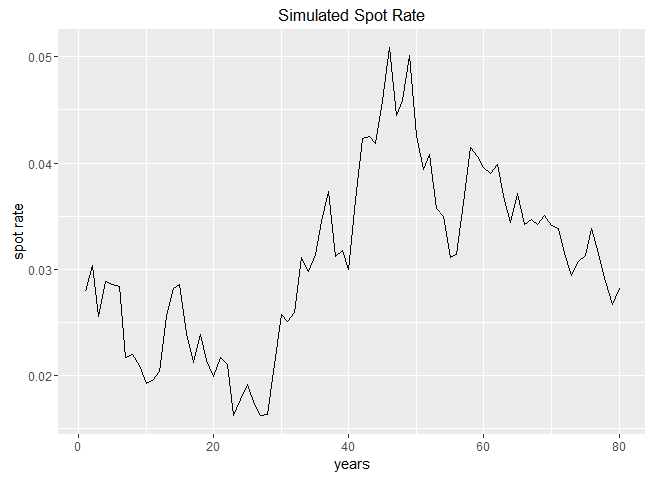
\includegraphics[height=0.4\textwidth,width=0.8\textwidth]{figure1}
			\caption{Simulated Spot Rate}
			\label{fige1}
		\end{figure}
	\end{frame}
	
	
	%15th page
	\begin{frame}
		\frametitle{Spot Rate Series and Term Structure}
		\framesubtitle{Term Structure implied by the estimated parameters}
		For the spot interest rate is greater than b, the term structure is as figure 2 shows, the yield reduces as the time to maturity increases.
		\begin{figure}[H]
			\centering
			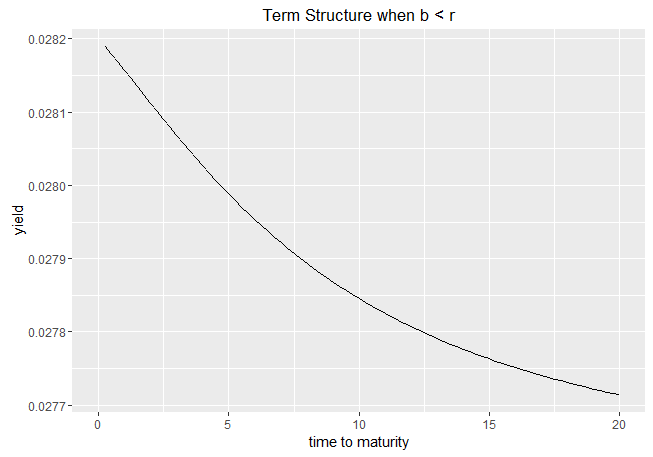
\includegraphics[height=0.4\textwidth,width=0.7\textwidth]{figure2}
			\caption{Term Structure with $ r(t)>b $}
			\label{fige2}
		\end{figure}
	\end{frame}
	
	
	%16th page
	\begin{frame}
		\frametitle{Spot Rate Series and Term Structure}
		\framesubtitle{Term Structure implied by the estimated parameters}
		For the spot interest rate is smaller than $ Y_{lim} $, the term structure is as figure 3 shows, the yield rises as the time to maturity increases.
		\begin{figure}[H]
			\centering
			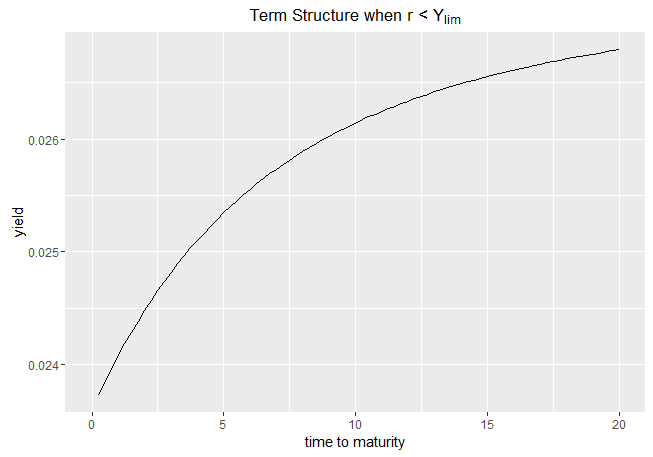
\includegraphics[height=0.4\textwidth,width=0.7\textwidth]{figure3}
			\caption{Term Structure with $ r(t)<Y_{lim} $}
			\label{fige3}
		\end{figure}
	\end{frame}
	
	
	%17th page
	\begin{frame}
		\frametitle{Spot Rate Series and Term Structure}
		\framesubtitle{Term Structure implied by the estimated parameters}
		For the spot interest rate is between b and $ Y_{lim} $, the term structure is as figure 4 shows, the term structure first rises and then falls.
		\begin{figure}[H]
			\centering
			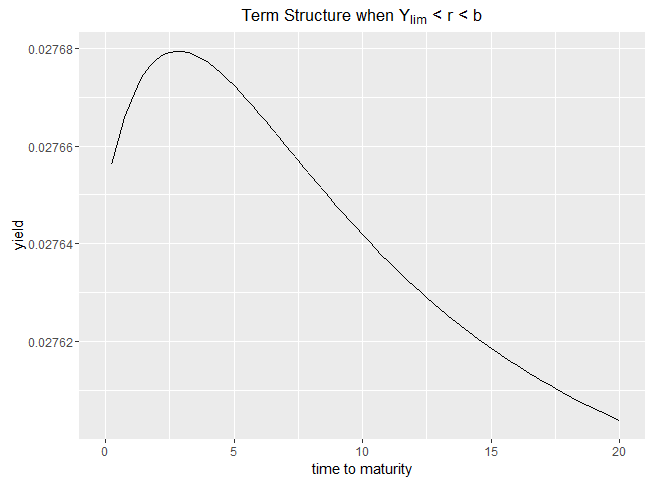
\includegraphics[height=0.4\textwidth,width=0.7\textwidth]{figure4}
			\caption{Term Structure with $ b>r(t)>Y_{lim} $}
			\label{fige4}
		\end{figure}
	\end{frame}

\end{document}
